\documentclass{article}

\usepackage{amsmath}
\usepackage{mathtools}
\usepackage{subfigure}
\setlength\parindent{0pt}

\setlength{\textwidth}{6.2in}
\setlength{\oddsidemargin}{0.0in}
\setlength{\evensidemargin}{0in}
\setlength{\textheight}{8.9in}
\setlength{\voffset}{-1in}
\setlength{\headsep}{26pt}
\setlength{\parindent}{0pt}
\setlength{\parskip}{5pt}

\begin{document}

\section{Introduction}
Kelsey
\section{LWR Model}
Kelsey
\section{PW Model}

\subsection{Theory}
Kelsey
\subsection{Hugoniot Loci and Integral Curves}
Brisa
\section{AR Model}

\subsection{Theory}
Kelsey
\subsection{Hugoniot Loci and Integral Curves}
The AR model starts from the system
\begin{align}
&\partial_t\rho + \partial_x(\rho v) = 0, \label{AW:eq1}\\
&\partial_t \left(v + p(\rho )\right) + v\partial_x \left( v + p(\rho )\right) = 0.
\end{align}

To find the Hugoniot loci and the integral curves, \cite{AwRascle2000} utilizes two different forms of this system. 
We will examine each of them in turn. What we will find is that the integral curves and the Hugoniot loci coincide, 
and furthermore that one of the waves is a contact discontinuity. Let us first consider the Hugoniot loci. 

\subsubsection{Hugoniot Loci}
In order to consider the Hugoniot loci for this system we must first write the system in conversation form. 
To accomplish this, note that multiplying the first equation by $(v + p(\rho ))$ and the second equation 
by $\rho$ gives us the two equations 
\begin{align*}
&(v + p(\rho ))\partial_t\rho + (v + p(\rho ))\partial_x(\rho v) = 0,  \\
&\rho\partial_t \left(v + p(\rho )\right) + \rho v\partial_x \left( v + p(\rho )\right) = 0.
\end{align*}
Adding these two equations gives
\begin{align}\label{AW:eq2}
\partial_t \left(\rho\left(v + p(\rho )\right)\right) + \partial_x \left( \rho v\left(v + p(\rho )\right)\right) = 0.
\end{align}
Then from (\ref{AW:eq1}) and (\ref{AW:eq2}) we have the system 
\begin{align*}
&\partial_t\rho + \partial_x(\rho v) = 0, \\
&\partial_t \left(\rho\left(v + p(\rho )\right)\right) + \partial_x \left( \rho v\left(v + p(\rho )\right)\right) = 0.
\end{align*}
This can be rewritten as $q_t + f(q)_x = $ by defining
\begin{align*}
q = \left[ \begin{matrix}
\rho \\ y
\end{matrix}\right], \hspace{0.3in}
f(q) = \left[ \begin{matrix}
v\rho \\
vy
\end{matrix}\right].
\end{align*}
where $y = \rho\left(v + p(\rho )\right)$.
The Rankine-Hugoniot condition tells us that 
\begin{align*}
s(q_*- q) = f(q_*) - f(q).
\end{align*}
Therefore, from this condition we get the two equations
\begin{align}
s(\rho_* - \rho) = v_*\rho_* - v\rho, \label{AW:eq3}\\
s(y_* - y) = v_*y_* - vy.\label{AW:eq4}
\end{align}
With a little rearranging and by plugging in for $y$, these two equations can be rewritten as
\begin{align}
&\rho_*(s - v_*) = \rho (s - v), \label{AW:eq5}\\
&\rho_*(s - v_*)\left(v_* + p(\rho_* )\right) = \rho(s - v)\left(v + p(\rho )\right).
\end{align}
From (\ref{AW:eq5}), we know that there are two cases: 

(a) $\rho_*(s - v_*) = \rho (s - v) = 0$. In this case we have that
\begin{align*}
s - v_* = s - v 
\end{align*}
except if one of the two densities, $\rho_*$, $\rho$ is zero. WHY DOES THIS NOT MATTER? Therefore, we can say that
\begin{align*}
v_* = v.
\end{align*}
Since the velocity does not change, this is a contact discontinuity. Using the fact that $v = v_*$ in (\ref{AW:eq4}) gives
\begin{align*}
y_*(s - v) = y(s - v).
\end{align*}
So, either $y = y_*$ or $s = v$. If $y = y_*$ we have a stationary point in the $Y = (\rho, y)$ plane, which does not 
describe a wave. Therefore, $s = v$. Note that we have no restrictions on $y$ other than its definition. 
Therefore this loci in the $Y$ plane is given by 
\begin{align*}
y = \rho ( v_* + p(\rho )).
\end{align*}
(b) $\rho_*(s - v_*) = \rho (s - v) \neq 0$. In this case, solving (\ref{AW:eq3}) for $s$ gives
\begin{align*}
s = \frac{\rho_*v_* - \rho v}{\rho_* - \rho}.
\end{align*}


\begin{figure}[h!]
 \centering
 \subfigure[$\lambda_1$-curves in the U plane.]{
  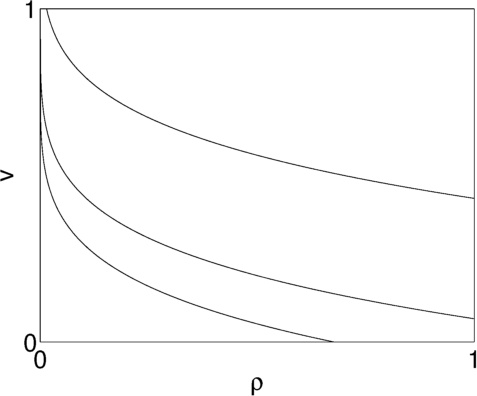
\includegraphics[width=45mm]{../MatlabCode/Images/HLIC_U_lamb1.jpg}
   \label{fig:subfig1}
   }
 \subfigure[$\lambda_2$-curves in the U plane.]{
  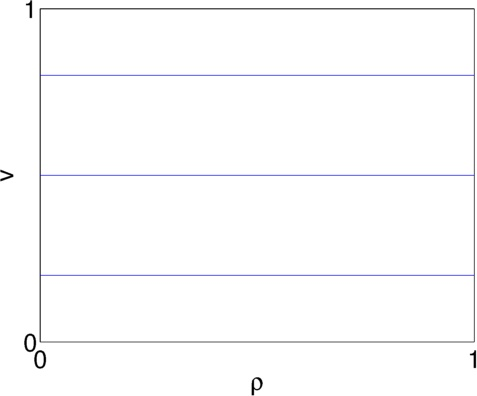
\includegraphics[width=45mm]{../MatlabCode/Images/HLIC_U_lamb2.jpg}
   \label{fig:subfig2}
   }
 \subfigure[$\lambda_1$-curve and $\lambda_2$-curve in the U plane passing through
  the point $(\rho_*, v_*)$ denoted by the red point.]{
  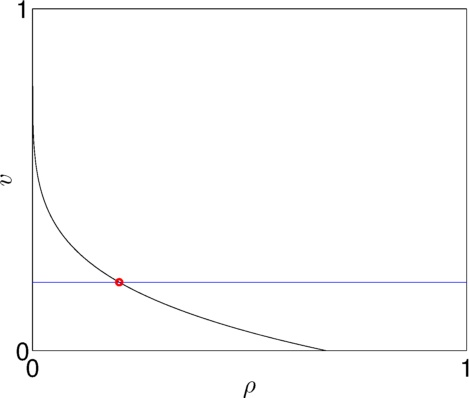
\includegraphics[width=45mm]{../MatlabCode/Images/HLIC_U.jpg}
   \label{fig:subfig3}
   }
    \subfigure[$\lambda_1$-curves in the M plane.]{
  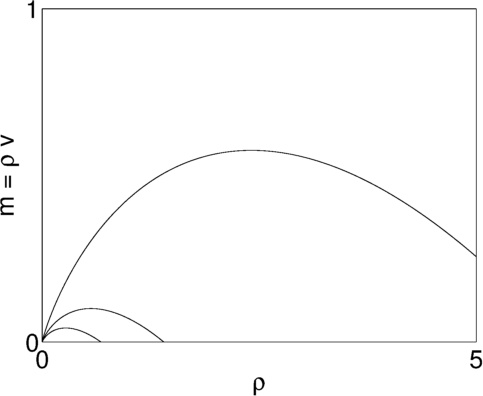
\includegraphics[width=45mm]{../MatlabCode/Images/HLIC_M_lamb1.jpg}
   \label{fig:subfig4}
   }
 \subfigure[$\lambda_2$-curves in the M plane.]{
  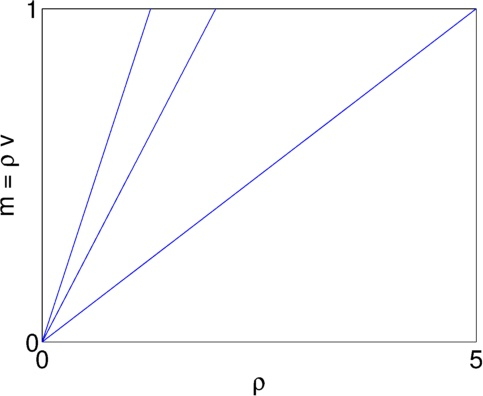
\includegraphics[width=45mm]{../MatlabCode/Images/HLIC_M_lamb2.jpg}
   \label{fig:subfig5}
   }
 \subfigure[$\lambda_1$-curve and $\lambda_2$-curve in the M plane passing through 
 the point $(\rho_*,m_*)$ denoted by the red point.]{
  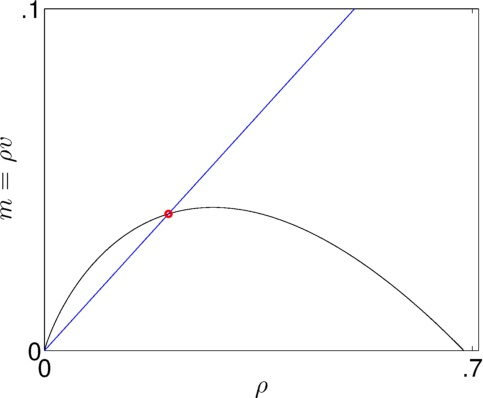
\includegraphics[width=45mm]{../MatlabCode/Images/HLIC_M.jpg}
   \label{fig:subfig6}
   }
       \subfigure[$\lambda_1$-curves in the Y plane.]{
  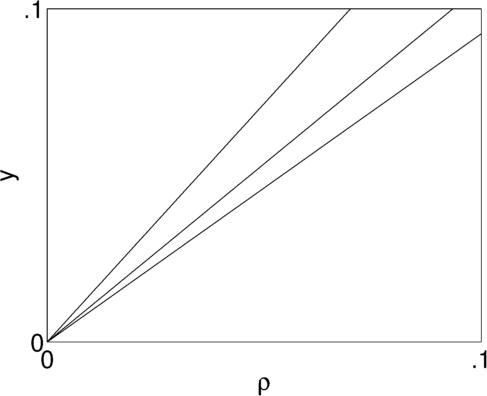
\includegraphics[width=45mm]{../MatlabCode/Images/HLIC_Y_lamb1.jpg}
   \label{fig:subfig7}
   }
 \subfigure[$\lambda_2$-curves in the Y plane.]{
  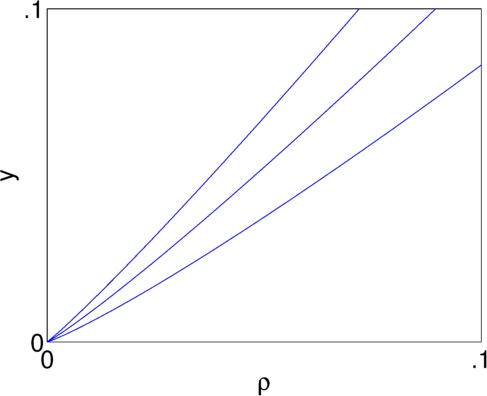
\includegraphics[width=45mm]{../MatlabCode/Images/HLIC_Y_lamb2.jpg}
   \label{fig:subfig8}
   }
 \subfigure[$\lambda_1$-curve and $\lambda_2$-curve in the Y plane passing through 
 the point $(\rho_*, y_*)$ denoted by the red point.]{
  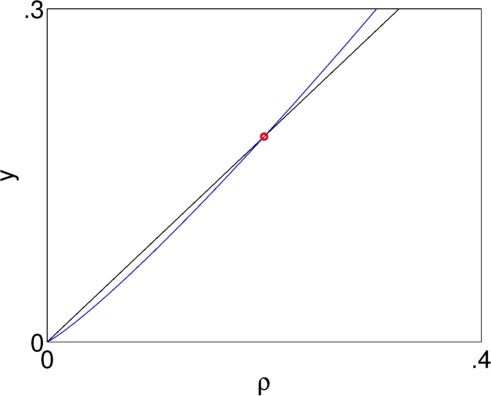
\includegraphics[width=45mm]{../MatlabCode/Images/HLIC_Y.jpg}
   \label{fig:subfig9}
   }
 \label{fig:11_8c}
 \caption[Optional caption for list of figures]
 {Figures of the Hugonio loci and integral curves for $\lambda_1$ and $\lambda_2$ 
 in each of the different planes. Since the loci and integral curves coincide, they are both
  simply called the ``curves'' in the captions of the above figures. Figures (c), (f), (i) show
   both curves for a given point in each plane.}
\end{figure}

\section{Examples}
Brisa

\bibliography{Draft}{}
\bibliographystyle{plain}
\end{document}